\documentclass[sigconf, timestamp-false, anonymous=true]{acmart}

\usepackage{listings}
\usepackage{multirow}

%% Rights management information.  This information is sent to you
%% when you complete the rights form.  These commands have SAMPLE
%% values in them; it is your responsibility as an author to replace
%% the commands and values with those provided to you when you
%% complete the rights form.
\setcopyright{none}

\acmConference[ESEC/FSE '20]{ESEC/FSE '20: ACM Joint European Software Engineering Conference and Symposium 
on the Foundations of Software Engineering}{November 8-13, 2020}{Sacramento, CA, USA}
\acmYear{2020}

\newcommand\todo[1]{\textcolor{red}{#1}}

%%
%% Submission ID.
%% Use this when submitting an article to a sponsored event. You'll
%% receive a unique submission ID from the organizers
%% of the event, and this ID should be used as the parameter to this command.
%%\acmSubmissionID{123-A56-BU3}

%%
%% The majority of ACM publications use numbered citations and
%% references.  The command \citestyle{authoryear} switches to the
%% "author year" style.

%%
%% end of the preamble, start of the body of the document source.
\begin{document}

\title{A Study of Multi-Edit Bug Patches}

%add authors & shortauthors if we are lucky :)

\begin{abstract}
  \todo{note that this is probably full of falsehoods, I'm just thinking by
    typing.} Automatic program repair is a promising approach for reducing the
    cost of quality assurance practices and faulty software. To date, most
    techniques proposed for test-driven automatic repair have succeeded
    primarily on bugs that benefit from short, single-edit patches. Techniques
    that succeed on multi-edit bugs often do so by patching them in an
    alternative, single-edit way, or by targeting particular multi-edit bug
    patterns. Empirical studies of real-world similarly tend to focus on the
    patterns exhibited by single-edit bugs, and have not examined repairability
    of multi-edit bugs in detail. We present a comprehensive empirical analysis
    of multi-edit bugs in open source Java programs, focusing on static and
    dynamic properties that define the repair search space for a given bug (and
    thus, in turn, the challenges that apply to automatically addressing them).
    This analysis focuses on the key challenges of the dynamic program repair
    problem: the \emph{mutations and fix code} used to repair multi-edit bugs;
    the \emph{fault locations} and their relationships; and the \emph{objective
      function}, and in particular how and to what degree test cases can be used
    (or not) to identify partial repairs. We identify key takeaways and
    challenges, with implications for future work in expressive, multi-chunk bug
    repair.
\end{abstract}

%%
%% The code below is generated by the tool at http://dl.acm.org/ccs.cfm.
%% Please copy and paste the code instead of the example below.
\begin{CCSXML}
<ccs2012>
<concept>
<concept_id>10011007.10011074.10011099.10011102</concept_id>
<concept_desc>Software and its engineering~Software defect analysis</concept_desc>
<concept_significance>500</concept_significance>
</concept>
<concept>
<concept_id>10011007.10011074.10011784</concept_id>
<concept_desc>Software and its engineering~Search-based software engineering</concept_desc>
<concept_significance>500</concept_significance>
</concept>
</ccs2012>
\end{CCSXML}

\ccsdesc[500]{Software and its engineering~Software defect analysis}
\ccsdesc[500]{Software and its engineering~Search-based software engineering}

\keywords{software bugs, program repair}

\maketitle

\section{Introduction}

Software bugs are hard. That's why we need automated program repair.

Many bugs require multiple chunks or parts of patches. For example, Sobreira et. al reports that over half of the bugs in Defects4J are patched by two or more chunks ~cite{d4j-dissection}. In Zhong and Su's empirical study of bugs in Apache projects, they found that 70\% of buggy source files required two or more repair actions~\cite{zhong2015}. \todo{(this is, however, different than multiple locations.)}

Despite the prevalence of multi-chunk bugs, much of the previous work on automated program repair works best on bugs with single location patches, as to avoid the combinatorial growth of the search space with multiple locations. For example, fault localization techniques often assume that a bug is localized if any one buggy line is identified~\cite{fl-survey-wong}. Program repair techniques are often most effective on bugs that have only a single repair location~\cite{rsrepair, ae, hdrepair}.

Work on multi-chunk bugs are often focused on code clones and syntactically similar code chunks~\cite{saha2019harnessing,jiang2019cmsuggester}. \todo{something about the empirical multi-entity paper?~\cite{wang2018}} \todo{some more citations from Zhen's intro~\cite{fl-multi-faults, patch-correctness, Le2018}}

In order to repair more complex multi-chunk bugs, we need to study their characteristics. In this work, we hope to look at the characteristics of multi-chunk bugs, with an eye to automatically repairing them.

We focus on three specific aspects -- fault localization, repair actions, and evaluation.


\section{Background}
\subsection{Automated Program Repair (APR)}
Automated program repair (APR) techniques aim to find patches for broken programs. 
Given a buggy program and an oracle for program correctness (e.g: test cases), APR 
techniques attempt to produce a series of edits that causes the program to satisfy the 
correctness oracle. 

A popular search-based repair technique is to treat program repair as an optimization 
problem, where the repair technique attempts uses a heuristic for patch quality to guide 
the search for a high quality patch within the space of possible patches. A popular heuristic
measure of patch quality is the number of passing test cases.

\subsection{Fault Localization}

Work on fault localization started in assisting human developers with debugging. When people started doing program repair, folks just plucked those techniques and used them for program repair. 

The most commonly used fault localization technique is Spectrum Based Fault Localization (SBFL). 

\section{Datasets}
We study bugs from Defects4J~\cite{defects4j} and Bears~\cite{bears}---datasets of 
bugs found in real world software projects.

Defects4J contains 438 bugs from six Java software projects. This  
is currently the most popular Java dataset for evaluating program repair tools~\cite{durieux-repair-them-all}.
Many such tools, however, overfit to Defects4J and perform worse on other 
benchmarks~\cite{durieux-repair-them-all}. 

Bears is a set of Java bugs derived from failed Travis-CI builds of GitHub projects.
Bears offers 251 bugs from 72 software projects, offering a greater diversity of 
projects compared to Defects4J.

\todo{can we have a description of chunk rules here (should be moving the stuff in partial repairs subsection), plus maybe a table or something about how many multichunk bugs there are?}

\section{Frequency of Multi-Edit Bugs}

\subsection{Research Question}

\textbf{RQ1: How many multi-edit patches are in Defects4J and Bears?}
We start our analysis of multi-edit patches by asking how many such patches 
exist in our benchmarks. We analyze edits at two levels: line and chunk.
Line edits include adding, deleting, or modifying lines.
Chunks are sequences of consecutive line edits.
We ignore whitespace and comments when counting edits.

\subsection{Results}

\begin{table}
{\begin{center}
	\begin{tabular}{l | rrrr | r}
		\toprule
		Dataset & 1-line & Multiline & 1-chunk & Multichunk & Total \\
		\midrule
		\multirow{ 2}{*}{Defects4J} & 92 & 303 & 298 & 97 & 395 \\
		& 23\% & 77\% & 75\% & 25\% & 100\% \\
		\multirow{ 2}{*}{Bears} & 31 & 150 & 117 & 64 & 181 \\
		& 17\% & 83\% & 65\% & 35\% & 100\% \\
		\midrule
		\multirow{ 2}{*}{Combined} & 123 & 453 & 415 & 161 & 576 \\
		& 21\% & 79\% & 72\% & 28\% & 100\% \\
		\bottomrule
	\end{tabular}
 \end{center}
}
	\caption{Frequencies and percentages of patches with multi-line and multi-chunk edits.}
	\label{tab:multiedit-frequencies}
\end{table}

Table~\ref{tab:multiedit-frequencies} lists the number and percentages of Defects4J and Bears
multi-line and multi-chunk patches.

\section{Fitness Experiment}

In search based program repair, one key area of research is to find ways to measure how "close" a candidate patch is to a full repair (a fitness function),
and this is usually done via measuring unit test performance of the candidate patch. 
Given a buggy program and a valid repair, if we apply a part of the valid repair to the buggy program (a partial repair), then semanticly the partial repair is closer to the full repair compared to the original. 
Ideally, we would want the fitness function to guide the search towards a full repair by identifying partial repairs as "closer" to full repair than original.
However, sometimes partial repairs will perform no different in unit tests compared to the original program, and other times they could perform worse. We want to find out how often each of these situations happen.

Moreover, unit test performance can be measured in different granularity levels. The most common ones used in existing APR tools are class level and method level. 
It is commonly believed that the more granular a fitness functions is, the better it is because it collects more information and is less likely to plateau. Thus, we introduce a third granularity level: assertion level, which is more granular than method level granularity.
We would like to compare the performance of the fitness functions at identifying partial repairs at different granularity levels.

The results may provide valuable information to future search-based program repair tool designs.

\subsection{Partial Repairs}

For each bug in Defects4j (excluding Clojure bugs) and Bears (single-module only), we look at the provided correct patch and divide it into edit chunks using the following steps:

1. Each consecutive block of edits (including both insertion and deletion) is labeled as one chunk.

2. Discard all edits that does not actually affect the program (such as comment change, fixing spaces, etc)

3. If a set of matched brackets that are both inserted or deleted in two different chunk, merge those two chunks into one; if a bracket is deleted in one chunk but inserted back in another chunk (matched to the same opposite bracket), merge these two chunks into one

4. We introduce a new set of edits, Base, initially empty. If a variable declaration is deleted, discard the deletion edit; if a variable declaration is inserted, move this edit to Base; if a variable declaration is moved upwards in code, move the variable moving edits to Base; if a variable declaration is moved downwards in code, discard the moving edits. Declaration modifications (i.e. changing parts of the variable declaration, but not the variable name or the location of the declaration), however, does not belong to any of the cases above.

5. Any insertion of imports or additional helper methods are moved to Base; any deletion of imports or helper methods is discarded

After the steps above, we count the number of remaining chunks (not including Base) and call it the chunk number of the bug, label the chunks with positive numbers, and make a power set of the chunks excluding the empty set and the complete set. Then, for each subset of the chunks, we apply all edits in chunks in this subset and Base to the original buggy code, and we define this as a partial repair. For a bug with chunk number n, it should have $2^n-2$ partial repairs. 

In this experiment, each edit chunk will be viewed as a single edit. Thus, only bugs with chunk number between 2 and 6 (inclusive) is selected, as bugs with chunk number more than 6 are rare but has too many partial repairs to evaluate.

Note that the reason of steps 4 and 5 is to make sure that all declarations are present in all partial repairs such that the partial repairs compile (thus can be tested). Since there are almost no cases where a declaration in patch have side effects, it is okay to include redundant variable/method declarations in partial repairs, as they will not affect the program's performance in unit tests. 

\subsection{Unit Testing Granularity}

There are different ways to compare unit test results, and the most common ways are class-level granularity and method-level granularity. At Class-level granularity, we only look at which test classes passed and which failed; at method-level granularity, we look at which test methods passed and which failed.

Here we introduce a third level of granularity: assertion-level granularity. For each test method $M$, let $A(M)$ be the set of all assert statements in $M$. When $M$ is run, if an assertion failed, the failure is recorded and the method is allowed to continue to run (as opposed to normally the test method throws an error and terminates). After running the method, for each assert statement $a\in A(M)$, let $b(a)$ be 1 if $a$ never failed once during the running of $M$, and 0 otherwise. We define the assertion score of $M$ to be $AS(M)=\frac{\Sigma_{a\in A(M)}b(a)}{|A(M)|}$. If $M$ failed to run to completion due to timeouts or exceptions that are not related to assertions, then we define $AS(M)=0$. Thus by definition, $AS(M)=1$ if $M$ passes. If a program passed more assertions in $M$, there should be an increase in $AS(M)$.

\subsection{Test Result Notations}

For each bug, run unit tests on all three levels of granularity on the original buggy code and all partial repairs. Then, the test results of each partial repair is compared to the test results of the original buggy code, and the comparison result is represented using one of the following labels (PR means partial repair, OBC means original buggy code):

\begin{tabular}{| l | l |}
\hline
  Label & Meaning \\
  
  \hline
  c+ & PR passed more test classes than OBC  \\\hline
  c- & PR passed less test classes than OBC  \\\hline
  m+ & PR and OBC passed same number of test classes, \\
  & PR passed more methods than OBC and passed all methods that OBC passed\\\hline
  m- & PR and OBC passed same number of test classes, \\
  & OBC passed more methods than PR and passed all methods that PR passed\\\hline
  m\~ & PR and OBC passed same number of test classes, \\
  & PR passed some methods that OBC didn't, \\
  & and OBC passed some methods that PR didn't \\\hline
  a+ & PR and OBC passed exact same test methods, \\
  & PR has higher assertion scores in some failed methods than OBC \\
  & and has equal assertion scores in all other failed methods \\\hline
  a- & PR and OBC passed exact same test methods, \\
  & PR has lower assertion scores in some failed methods than OBC \\
  & and has equal assertion scores in all other failed methods \\\hline
  a\~ & PR and OBC passed exact same test methods, \\
  & PR has higher assertion scores in some failed methods than OBC \\
  & and has lower assertion scores in some other failed methods \\\hline
  0 & PR and OBC passed exact same test methods \\
  & and has same assertion score for all failed methods \\ \hline
  NC & PR did not compile \\\hline
 
  
\end{tabular}


\subsection{Unminimized Results}

After doing the steps in section 2.1, there are 97 bugs in Defects4j and 64 bugs in Bears that has chunk number between 2 and 6. Since each bug may have different number of partial repairs, we analyzed the results in two different ways: Unweighted (where each partial repair has weight 1), and weighted (where each bug has a total weight of 1, so if a bug has n partial repairs each of them has weight $\frac{1}{n}$). Here is the full result:

\begin{tabular}{| l | l | l | l | l |} \hline
    Dataset & Defects4j & Defects4j & Bears & Bears  \\ \hline
    Weightedness & Unweighted & Weighted & Unweighted & Weighted \\ \hline
    Total & 898 & 97 & 444 & 64 \\ \hline
    c+ & 102 & 19.84 & 129 & 17.67 \\
    c- & 108 & 6.97 & 18 & 4.29 \\
    m+ & 216 & 20.16 & 38 & 2.36 \\
    m- & 65 & 5.18 & 4 & 1 \\
    m~ & 1 & 0.07 & 0 & 0 \\
    a+ & 45 & 6.79 & 6 & 0.2 \\
    a- & 23 & 0.37 & 21 & 1.94 \\
    a~ & 13 & 0.21 & 1 & 0.5 \\
    0 & 248 & 30.77 & 219 & 30.39 \\
    NC & 77 & 6.62 & 8 & 1.67 \\
    \hline
    
    
    \end{tabular}
    
    Thus, from the data above, we can compute the percentage of partial repairs that are identified positively by each granularity level:
    
    \begin{tabular}{| l | l | l | l | l |} \hline
    Dataset & Defects4j & Defects4j & Bears & Bears  \\ \hline
    Weightedness & Unweighted & Weighted & Unweighted & Weighted \\ \hline
    Class Level Granularity & 11.36\% & 20.46\% & 29.05\% & 27.60\%\\
    Method Level Granularity & 35.41\% & 41.25\% & 37.61\% & 31.29\% \\
    Assertion Level Granularity & 40.42\% & 48.25\% & 38.96 \% & 31.60\% \\
    \hline
    
    \end{tabular}

    Here are the percentage of partial repairs that performs no different at each granularity level:
    
    \begin{tabular}{| l | l | l | l | l |} \hline
    Dataset & Defects4j & Defects4j & Bears & Bears  \\ \hline
    Weightedness & Unweighted & Weighted & Unweighted & Weighted \\ \hline
    Class Level Granularity & 68.04\% & 65.53\% & 65.09\% & 56.84\%\\
    Method Level Granularity & 36.64 \% & 39.33\% & 55.63\% & 51.60\% \\
    Assertion Level Granularity & 27.62\% & 31.73\% & 49.32 \% & 47.48\% \\
    \hline
    
    \end{tabular}
    
    Here are the percentage of partial repairs that performed worse compared to original buggy program at each granularity level:
    
    \begin{tabular}{| l | l | l | l | l |} \hline
    Dataset & Defects4j & Defects4j & Bears & Bears  \\ \hline
    Weightedness & Unweighted & Weighted & Unweighted & Weighted \\ \hline
    Class Level Granularity & 12.03\% & 7.18\% & 4.05\% & 6.70\%\\
    Method Level Granularity & 19.27 \% & 12.52\% & 4.95\% & 8.26\% \\
    Assertion Level Granularity & 21.83\% & 12.90\% & 9.68 \% & 11.29\% \\
    \hline
    
    \end{tabular}
    
    

\subsection{Minimized Results}

During the experiment, we found that sometimes not all edit chunks of a bug is necessary to pass all tests, because one or more of its partial repairs passed all tests. This means that some chunks in the provided correct patch is redundant. 

Sicne we're only interested in edits that are necessary for the repair, we processed the data to ignore redundant chunks and all partial repairs that included them. 32 out of 97 defects4j bugs and 34 out of 64 Bears bugs are affected. Some bugs ends up with chunk number 1 after minimization, so they are not included in the Minimized results. The minimized results include 75 remaining bugs in defects4j and 38 remaining bugs of Bears.

\begin{tabular}{| l | l | l | l | l |} \hline
    Dataset & Defects4j & Defects4j & Bears & Bears  \\ \hline
    Weightedness & Unweighted & Weighted & Unweighted & Weighted \\ \hline
    Total & 566 & 75 & 156 & 38 \\ \hline
    c+ & 30 & 7.33 & 19 & 4.02 \\
    c- & 56 & 5.73 & 17 & 4.12 \\
    m+ & 167 & 20.26 & 18 & 3.47 \\
    m- & 44 & 4.86 & 0 & 0 \\
    m~ & 1 & 0.07 & 0 & 0 \\
    a+ & 31 & 6.83 & 6 & 0.2 \\
    a- & 5 & 0.19 & 13 & 1.67 \\
    a~ & 10 & 0.22 & 1 & 0.5 \\
    0 & 181 & 22.73 & 77 & 22.49 \\
    NC & 41 & 5.77 & 5 & 1.83 \\
    \hline
    
    
    \end{tabular}
    
    Thus, from the data above, we can compute the percentage of partial repairs that are identified positively by each granularity level:
    
    \begin{tabular}{| l | l | l | l | l |} \hline
    Dataset & Defects4j & Defects4j & Bears & Bears  \\ \hline
    Weightedness & Unweighted & Weighted & Unweighted & Weighted \\ \hline
    Class Level Granularity & 5.30\% & 9.78\% & 12.18\% & 10.59\%\\
    Method Level Granularity & 34.81\% & 36.80\% & 23.72\% & 19.71\% \\
    Assertion Level Granularity & 40.28\% & 45.91\% & 27.56 \% & 20.24\% \\
    \hline
    
    \end{tabular}

    Here are the percentage of partial repairs that performs no different at each granularity level:
    
    \begin{tabular}{| l | l | l | l | l |} \hline
    Dataset & Defects4j & Defects4j & Bears & Bears  \\ \hline
    Weightedness & Unweighted & Weighted & Unweighted & Weighted \\ \hline
    Class Level Granularity & 77.56\% & 73.56\% & 73.72\% & 73.75\%\\
    Method Level Granularity & 40.11 \% & 39.95\% & 62.18\% & 64.62\% \\
    Assertion Level Granularity & 31.98\% & 30.30\% & 49.36 \% & 59.19\% \\
    \hline
    
    \end{tabular}
    
    Here are the percentage of partial repairs that performed worse compared to original buggy program at each granularity level:
    
    \begin{tabular}{| l | l | l | l | l |} \hline
    Dataset & Defects4j & Defects4j & Bears & Bears  \\ \hline
    Weightedness & Unweighted & Weighted & Unweighted & Weighted \\ \hline
    Class Level Granularity & 9.89\% & 7.64\% & 10.90\% & 10.84\%\\
    Method Level Granularity & 17.67 \% & 14.13\% & 10.90 \% & 10.84\% \\
    Assertion Level Granularity & 18.55 \% & 14.39 \% & 19.23 \% & 14.44\% \\
    \hline
    
    \end{tabular}
    
\subsection{Interpretations}

1. As expected, the more granular the fitness function gets, the more likely a partial repair gets identified positively or negatively.

2. In both datasets, method level granularity performed a lot better than class level granularity. Assertion level granularity performed better than method level granularity in Defects4j (significant increase in positively identifying partial repairs and minimal increase in negatively identifying partial repairs) and not so well in Bears (almost no increase in positively identifying partial repairs while significantly increasing negatively identifying partial repairs).

3. In general, it seems that unit test results are less sensitive to granularity level in Bears compared to Defects4j. Fitness function with class level granularity performs approximately the same on both datasets in minimized results (and in unminimized results it actually did better in Bears), but as we get more granular, the fitness functions performs much better with Defects4j bugs compared to Bears bugs in both minimized and unminimized results.

\subsection{Limitations}

This experiment breaks up full repairs into chunks and treats each chunk as a single edit action. However, in reality most APR techniques edits a line or part of a line at a time. Also, this experiment only checks whether fitness functions can identify partial repairs, and not concerned with how to come up with these partial repairs (depending on specifics of the APR techniques, some may not be in the search space).

Regardless of its limitations, this experiment is provides valid and valuable information to tackling the challenge of automatically repairing bugs that requires multiple edit actions to fully repair and provides insight in future APR research.

\subsection{Relations between fitness experiment result and fault localization experiment result}

(I'm not sure where these findings belong to (or even if they should be in the paper), so I just toss them here for now)

Negative fitness tend to happen in "Same" category of coverage (8 out of 12 bugs has some partial repair that is negative, another 2 have all their partial repairs as 0). In bugs of category "Overlap" or "Disjoint", all of them has some partial repairs that results in more test methods passed, while only 5 out of 12 "Same" bugs has any partial repair that performs better than original. Moreover, "Disjoint" and "Overlap" category has very few partial repairs that has negative fitness compared to original: only 2 out of 17 Disjoint bugs has some negative partial repair, and only 1 out of 10 Overlap bugs have some negative partial repair. These results are kind of intuitive (we would expect multiple edits in the same location to cause more problems for partial repairs than Disjoint ones)

\section{Dependency Analysis}

The presence of control or data dependencies in a patch's edits 
indicates coupling between the dependent edits.
Such coupled edits might need to be repaired simultaneously.
\todo{Some motivating examples might be nice.}
We analyze control and data dependencies in bug patches along 
with their relationship to APR tool success.

\subsection{Research Questions}

RQ1: How many multi-edit patches contain control or data dependencies?

RQ2: Are bugs with dependent edits in the human patch more difficult to automatically repair?

\subsection{Methodology}

A patch contains dependent edits if there exists control or data dependencies 
between added, removed, or changed lines in the pre- or post-patch
source code. For practical reasons, we perform intraprocedural analysis, 
although we heuristically consider function arguments as reads 
and invocations of getter and setter methods as reads and writes.

\subsection{Results}

\begin{table}
{\begin{center}
	\begin{tabular}{l | rrrr | r}
		\toprule
		Dataset & Control & Data & Either & Neither & Total \\
		\midrule
		Defects4J & 123 & 78 & 132 & 171 & 303 \\
		& 40\% & 26\% & 44\% & 56\% & 100\% \\
		Bears & 83 & 63 & 95 & 55 & 150 \\
		& 53\% & 42\% & 63\% & 37\% & 100\% \\
		\midrule
		Combined & 206 & 141 & 227 & 226 & 453 \\
		& 45\% & 31\% & 50\% & 50\% & 100\% \\
		\bottomrule
	\end{tabular}
 \end{center}
}
	\caption{Frequencies of multi-line patches with control and data dependent line edits.}
	\label{tab:dependency}
\end{table}

\subsubsection{RQ1} Table~\ref{tab:dependency} shows the 
frequencies and percentages of multi-line patches with control or data dependent 
line edits. We find a higher proportion of dependent patches in Bears compared to 
Defects4J, indicating higher patch complexity among multi-line patches in Bears.


\begin{table}
{\begin{center}
	\begin{tabular}{l | l | r r r r | r}
		\toprule
		Dataset & APR & Control & Data & Either & Neither & Total \\
		\midrule
		\multirow{2}{*}{Defects4J} & Success & 34 & 21 & 39 & 94 & 133 \\
		                                          & Failure   &  89 & 57 & 93 & 77 & 170 \\
		\multirow{2}{*}{Bears}       & Success &    7 &   6 &   9 &   7 &   16 \\
		                                          & Failure   &  76 & 57 & 86 & 48 & 134 \\
		\midrule
		\multirow{2}{*}{Combined}& Success &  41 & 27 & 48 &101& 149 \\
		                                          & Failure   &165 &114&179&125& 304 \\
	\end{tabular}
 \end{center}
}
	\caption{Frequency of multi-line patches with respect to the presence of 
	control/data dependent line edits and whether an APR tool successfully 
	repaired the bug in~\cite{durieux-repair-them-all}.}
	\label{tab:dependency-repair-contingency-table}
\end{table}

\begin{table}
{\begin{center}
	\begin{tabular}{l | rrr}
            	\toprule
		& Defects4J & Bears & Combined \\
		\midrule
		$P(\mbox{APR Success } | \mbox{ Control})$ & 28\% &  8\% & 20\% \\
		$P(\mbox{APR Success } | \neg \mbox{ Control})$ & 55\% & 13\% & 44\% \\
		$P(\mbox{APR Success } | \mbox{ Data})$ & 27\% & 10\% & 19\%\\
		$P(\mbox{APR Success } | \neg \mbox{ Data})$ & 50\% & 11\% & 39\% \\
		$P(\mbox{APR Success } | \mbox{ Either})$ & 30\% & 9\% & 21\% \\
		$P(\mbox{APR Success } | \mbox{ Neither})$ & 45\% & 13\% & 45\% \\
		\bottomrule
	\end{tabular}
 \end{center}
}
	\caption{Percentages of auto-repaired bugs in~\cite{durieux-repair-them-all} 
	that (do not) contain control/data dependent line edits.}
	\label{tab:dependency-repair-percents}
\end{table}

\subsubsection{RQ2} 

Table~\ref{tab:dependency-repair-contingency-table} shows
the frequencies of multi-line patches with respect to the presence of 
dependent edits and whether an APR tool successfully auto-repaired the bug in~\cite{durieux-repair-them-all}.
Using $\chi^2$ tests, we find statistically significant relationships between APR  
success and control, data, and the disjunction of either dependencies 
($p < 0.001$ for all).
We find that bugs whose human patches are free of dependencies are
more likely to be successfully fixed by an APR tool.

Tables~\ref{tab:dependency-repair-contingency-table} and~\ref{tab:dependency-repair-percents}
show the frequencies and percentages of multi-line patches with respect to edit dependency 
and whether an APR tool successfully repaired bug in~\cite{durieux-repair-them-all}.
We find that edit dependency generally reduces the likelihood of APR tool success.
Using $\chi^2$ tests, we find statistically significant relationships ($p < 0.001$ for all)
between APR success and control, data, and the disjunction of either dependencies 
for Defects4J and Defects4J $\cup$ Bears patches. We fail to find statistically 
significant relationships over only Bears patches, possibly due to the small number (16) of 
successfully auto-repaired Bears bugs with multi-line human patches.


\section{Fault localization}

%% what are the claims, what are we studying, why are we studying it


Spectrum-based fault localization (SBFL) is the most commonly studied, as well as the most 
effective~\cite{zou2019empirical}, fault localization technique. It is a key
first step to characterizing the \emph{fault space} in automatic program repair,
narrowing the search space to a portion of the program more likely (based on
test case behavior) to correspond to the fault.  

\paragraph{SBFL Basics.} \todo{Serena, please add an explanation of how SBFL
  works; it's key to understanding the underlying assumption.  This should
  include references as appropriate.}

Given these basics, fundamentally, a core
assumption underlying SBFL is that \emph{failing tests execute buggy portions of 
the code relatively more often than passing tests.} Thus, if all failing tests execute a 
particular line of code, then that line of code is scored as more suspicious.
This assumption is well-suited to single edit repair. Indeed, the evaluation
of most SBFL techniques asks exactly the question of interest when considering a
technique's suitability for single-edit repair: how often does a given technique
correctly, highly rank individual buggy lines of code? 

Such evaluations, by and large, do not consider the implications of
suspeciousness scoring in a multi-edit repair context.  Instead, evaluations
typically consider a technique ``successful'' if it identifies \emph{any} of a
set of changed lines as highly-ranked or likely-suspicious.  While appropriate
for the question being asked in such evaluations, this does not address
suitability for multi-line program repair.  Identifying one of several buggy
locations is generally inadequate in a context where multiple locations must be
modified.  

Thus, in this research question, we investigate how well the SBFL assumption
applies to tests that identify multi-line bugs. We focus especially on
multi-line bugs that are associated with multiple tests; \todo{short explanation
  of the intuition why. This is a placeholder, I'm a bit tired and so this
  succinct explanation is escaping me.} If multiple tests all cover the multiple
modified locations well, then SBFL's core assumption holds and multi-edit repair
can expect to effectively make use of the off-the-shelf ranking these techniques
currently provide (indeed, this has been tried~\cite{angelix}). If not---that
is, if multiple tests exercise \emph{different} portions of the buggy
code---SBFL off-the-shelf will by definition be less effective in guiding APR to
correctly modifying multiple buggy locations at once.

Therefore, for multi-edit bugs with multiple identifying failing tests, do the 
different failing tests cover exactly the same patch locations, exactly 
disjoint path locations, or some combination?


\rqorinsight[2]{How well do multiple tests cover the multiple locations
  implicated in multi-edit bugs?}

\paragraph{Methodology}

Between both datasets, there are 60 total bugs that are both multi-edit and 
multi-test -- 45 in Defects4J and 15 in Bears. For each of these bugs, we used 
Jacoco to determine which of the chunks in the human patch were executed by each failing test. Using 
this coverage data, we categorized the bug as one of 
three coverage patterns: \textit{disjoint} for bugs in which no chunk is covered by all failing tests, 
\textit{same} for bugs in which all 
tests cover the exact same chunks of the patch, and \textit{overlap} for all 
other bugs, where some chunks are covered by all failing tests, but some chunks are only covered by a 
subset of failing tests.

\paragraph{Results}
The overall distribution is seen in Figure \ref{fig:coverage-all}. Over a third 
of the bugs were classified as disjoint, indicating that for a significant 
portion of bugs, the failing tests do not all execute any portion of the faulty 
code. In addition, another 22\% were classified as overlap. Thus, over half of 
the bugs that were both multi-edit and multi-test contained chunks that were 
not executed by all failing test cases.
2

\begin{figure}
	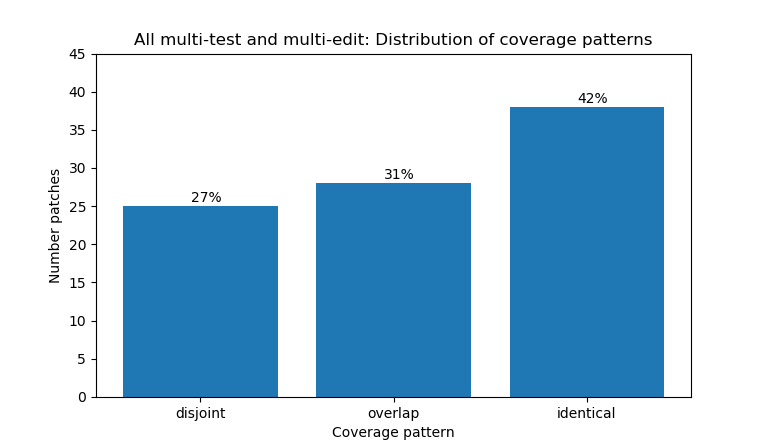
\includegraphics[width=\linewidth]{img/coverage-all.png}
	\caption{Distribution of coverage patterns for all multi-test and 
	multi-edit bugs in Bears and Defects4J. In all, 38\% of bugs were classified as disjoint, 40\% were 
	classified as same, and 22\% were classified as overlap.}
	\label{fig:coverage-all}
\end{figure}

SBFL assumes that faulty locations are executed more often by identifying 
or failing test cases and is not designed to find faults like these. Since SBFL 
is the most common fault localization technique in APR, most APR techniques 
are not well suited to fix a majority of these multi-edit and multi-test 
bugs.

If we divide distribution by dataset, we can see even more interesting 
behavior. Figure \ref{fig:coverage-datasets} shows the Defects4J dataset and 
the Bears dataset have very different distributions with respect to the 
disjoint and same categories -- in Defects4J, 47\% of bugs are disjoint and 
31\% are same, whereas in Bears, the proportions are 13\% disjoint and 67\% 
same. We hypothesize that this may be due to differences in how the two 
datasets were minimized, since Defects4J is a dataset of minimized and curated 
bugs while the bugs in Bears are taken scraped directly from the commits.


\begin{figure}
	\begin{subfigure}{\linewidth}
		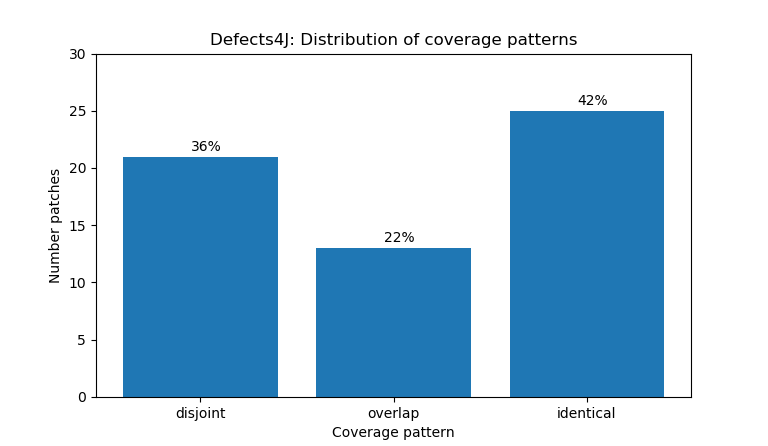
\includegraphics[width=\linewidth]{img/coverage-d4j.png}
		\caption{Distribution of coverage patterns for Defects4J. 47\% disjoint, 31\% same, and 22\% 
		overlap.}
	\end{subfigure}
	\begin{subfigure}{\linewidth}
		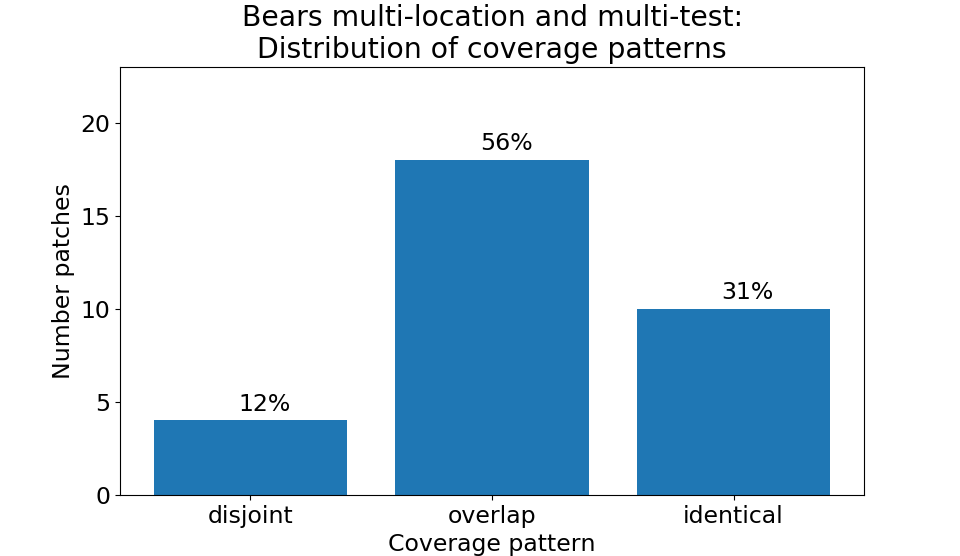
\includegraphics[width=\linewidth]{img/coverage-bears.png}
		\caption{Distribution of coverage patterns for Defects4J. 13\% disjoint, 67\% same, and 20\% 
		overlap.}
	\end{subfigure}
	\caption{Distribution of coverage patterns divided by dataset.}
	\label{fig:coverage-datasets}
\end{figure}


%\section{Symptoms}

We want to study symptoms in the context of fault localization. We define symptoms as the output given in failing test cases. In Java, most of these symptoms will be exceptions and their accompanying error message. Since most program repair is based off of failing tests, we want to see if those symptoms exhibited in those tests can correlate to type of repair.

For this paper, we specifically wanted to look at whether symptoms correlated with whether a bug could be fixed in a single location or multiple locations. If we can classify which bugs are single edit or multi edit, we can choose fault localization or patch generation techniques that are more suited.

We looked at all symptoms for all bugs in Defects4J and Bears, and categorized them based on whether they were one of the identified multi-chunk bugs or not. Then we fit the data to a linear regression model to see if there were statistically significant differences between the type of symptoms for multi edit and single edit bugs.

In order to find statistical significance, we needed to categorize the symptoms in big enough categories. We experimented with three groupings:

\begin{enumerate}
	\item Group all exceptions together except for assertion exceptions and exceptions for which a message indicates some sort of assertion (in our case, we simply looked for the keyword "expected"). We grouped the assertions into a few different types: 
	\begin{itemize}
		\item \lstinline{assert_null} is when the assertion is either expecting null, or got null when it wasn't expecting it.
		\item \lstinline{assert_int} is when the failing assertion was expecting a particular int value.
		\item \lstinline{assert_float} is the same as above, but for floats.
		\item \lstinline{assert_obj_arr_date} is when the assertion is expecting an object address, array of objects, or date object/date string. These are grouped together as commonly found but more complex assertions.
		\item \lstinline{error_expected} is when the failing test expected an exception, error, or warning.
		\item \lstinline{timeout} is when a Junit test times out, but also includes errors like stack overflows or out of memory exceptions.
		\item \lstinline{other_assert} for any other assertion that I couldn't easily categorize or parse. The large bulk of bugs in this category are bugs that had no error message at all; it simply failed with an \lstinline{AssertionError} or \lstinline{StackOverflow}.
		\item \lstinline{other}: all non-assertion exceptions.
	\end{itemize}
	\item Grouping symptoms together in an ad hoc way \todo{sell it better.}
	\begin{itemize}
		\item \lstinline{assert_prim}: assertions that compare to a Java primitive, such as int, float, or boolean.
		\item \lstinline{assert_null}: either expected or actual is null
		\item \lstinline{other_assert}: Asserting to anything that's not clearly a primitive or null.
		\item \lstinline{access}: all the bugs pertaining to wrongfully accessing or invoking certain fields or methods, or problems with classpath.
		\item \lstinline{null_pointer}: null pointer exceptions.
		\item \lstinline{timeout}: when a Junit test times out, but also includes errors like stack overflows or out of memory exceptions.
		\item \lstinline{parsing}: Anything related to parsing, serialization, or type conversion.
		\item \lstinline{other}: everything else
	\end{itemize}
	\item This last grouping is an even coarser version of the previous grouping.
	\begin{itemize}
		\item \lstinline{assert_equal}: Any assertion in which the test expected one value but got another
		\item \lstinline{other_assert}: any other assertion
		\item \lstinline{access}: all the bugs pertaining to wrongfully accessing or invoking certain fields or methods, or problems with classpath.
		\item \lstinline{null_pointer}: null pointer exceptions.
		\item \lstinline{parsing}: Anything related to parsing, serialization, or type conversion.
		\item \lstinline{other}: everything else
	\end{itemize}
\end{enumerate}

\todo{raw data from bogdan:}

assert only
\begin{lstlisting}
Call:
glm(formula = multi ~ assert_obj_arr_date + assert_int + assert_float + 
error_expected + timeout + assert_null + other_assert + other, 
family = "binomial", data = symptoms)Deviance Residuals: 
Min       1Q   Median       3Q      Max  
-1.2466  -0.5686  -0.4691  -0.4394   2.2880  Coefficients:
Estimate Std. Error z value Pr(>|z|)    
(Intercept)             -2.37550    0.38061  -6.241 4.34e-10 ***
assert_obj_arr_dateTRUE  1.24082    0.50907   2.437   0.0148 *  
assert_intTRUE           0.08619    0.45621   0.189   0.8502    
assert_floatTRUE         2.31273    0.48580   4.761 1.93e-06 ***
error_expectedTRUE       0.36735    0.53943   0.681   0.4959    
timeoutTRUE              0.99295    0.65378   1.519   0.1288    
assert_nullTRUE         -0.16611    0.58071  -0.286   0.7748    
other_assertTRUE         0.22402    0.36136   0.620   0.5353    
otherTRUE                0.63507    0.38201   1.662   0.0964 .  
---
Signif. codes:  0 '***' 0.001 '**' 0.01 '*' 0.05 '.' 0.1 ‘ ’ 1(Dispersion parameter for binomial family taken to be 1)    Null deviance: 546.49  on 645  degrees of freedom
Residual deviance: 510.11  on 637  degrees of freedom
AIC: 528.11Number of Fisher Scoring iterations: 5
\end{lstlisting}

grouping 1
\begin{lstlisting}
Call:
glm(formula = multi ~ access + assert_prim + null_pointer + timeout + 
assert_null + parsing + other_assert + other, family = "binomial", 
data = symptoms)Deviance Residuals: 
Min       1Q   Median       3Q      Max  
-0.9771  -0.6792  -0.5070  -0.4031   2.5944  Coefficients:
Estimate Std. Error z value Pr(>|z|)    
(Intercept)      -1.94778    0.36198  -5.381 7.41e-08 ***
accessTRUE        0.62756    0.41197   1.523   0.1277    
assert_primTRUE   0.81567    0.36223   2.252   0.0243 *  
null_pointerTRUE  0.32833    0.52496   0.625   0.5317    
timeoutTRUE       0.64782    0.63743   1.016   0.3095    
assert_nullTRUE  -0.52160    0.57971  -0.900   0.3682    
parsingTRUE       0.64081    0.50451   1.270   0.2040    
other_assertTRUE -0.03905    0.34777  -0.112   0.9106    
otherTRUE        -1.38263    0.76326  -1.811   0.0701 .  
---
Signif. codes:  0 '***' 0.001 '**' 0.01 '*' 0.05 '.' 0.1 ‘ ’ 1(Dispersion parameter for binomial family taken to be 1)    Null deviance: 546.49  on 645  degrees of freedom
Residual deviance: 523.84  on 637  degrees of freedom
AIC: 541.84Number of Fisher Scoring iterations: 5
\end{lstlisting}

grouping 2
\begin{lstlisting}
Call:
glm(formula = multi ~ assert_equal + access + null_pointer + 
parsing + other_assert + other, family = "binomial", data = symptoms)Deviance Residuals: 
Min       1Q   Median       3Q      Max  
-0.9390  -0.6809  -0.4377  -0.4377   2.2494  Coefficients:
Estimate Std. Error z value Pr(>|z|)    
(Intercept)       -2.0821     0.3470  -6.001 1.96e-09 ***
assert_equalTRUE   0.7532     0.3333   2.260   0.0238 *  
accessTRUE         0.7259     0.3979   1.824   0.0681 .  
null_pointerTRUE   0.4338     0.5131   0.845   0.3979    
parsingTRUE        0.7385     0.4976   1.484   0.1378    
other_assertTRUE  -0.2150     0.3223  -0.667   0.5048    
otherTRUE         -0.3646     0.5068  -0.719   0.4719    
---
Signif. codes:  0 '***' 0.001 '**' 0.01 '*' 0.05 '.' 0.1 ‘ ’ 1(Dispersion parameter for binomial family taken to be 1)    Null deviance: 546.49  on 645  degrees of freedom
Residual deviance: 527.48  on 639  degrees of freedom
AIC: 541.48Number of Fisher Scoring iterations: 5
\end{lstlisting}

In assert only, \lstinline{assert_float} correlates strongly with multiedit bugs. However, all the instances of \lstinline{assert_float} as a symptom occur in the Math package for Defects4J, and they all somehow to be multichunk. The sampling of \lstinline{assert_float} can be seenin the other two groupings as well, where \lstinline{asset_prim} and \lstinline{assert_equal}, both of which subsume \lstinline{assert_float}, are both more likey to be multi-edit.  \todo{take out math, redo analysis?}




\section{Symptoms}

We want to study symptoms in the context of fault localization. We define symptoms as the output given in failing test cases. In Java, most of these symptoms will be exceptions and their accompanying error message. Since most program repair is based off of failing tests, we want to see if those symptoms exhibited in those tests can correlate to type of repair.

For this paper, we specifically wanted to look at whether symptoms correlated with whether a bug could be fixed in a single location or multiple locations. If we can classify which bugs are single edit or multi edit, we can choose fault localization or patch generation techniques that are more suited.

We looked at all symptoms for all bugs in Defects4J and Bears, and categorized them based on whether they were one of the identified multi-chunk bugs or not. Then we fit the data to a linear regression model to see if there were statistically significant differences between the type of symptoms for multi edit and single edit bugs.

In order to find statistical significance, we needed to categorize the symptoms in big enough categories. We experimented with three groupings:

\begin{enumerate}
	\item Group all exceptions together except for assertion exceptions and exceptions for which a message indicates some sort of assertion (in our case, we simply looked for the keyword "expected"). We grouped the assertions into a few different types: 
	\begin{itemize}
		\item \lstinline{assert_null} is when the assertion is either expecting null, or got null when it wasn't expecting it.
		\item \lstinline{assert_int} is when the failing assertion was expecting a particular int value.
		\item \lstinline{assert_float} is the same as above, but for floats.
		\item \lstinline{assert_obj_arr_date} is when the assertion is expecting an object address, array of objects, or date object/date string. These are grouped together as commonly found but more complex assertions.
		\item \lstinline{error_expected} is when the failing test expected an exception, error, or warning.
		\item \lstinline{timeout} is when a Junit test times out, but also includes errors like stack overflows or out of memory exceptions.
		\item \lstinline{other_assert} for any other assertion that I couldn't easily categorize or parse. The large bulk of bugs in this category are bugs that had no error message at all; it simply failed with an \lstinline{AssertionError} or \lstinline{StackOverflow}.
		\item \lstinline{other}: all non-assertion exceptions.
	\end{itemize}
	\item Grouping symptoms together in an ad hoc way \todo{sell it better.}
	\begin{itemize}
		\item \lstinline{assert_prim}: assertions that compare to a Java primitive, such as int, float, or boolean.
		\item \lstinline{assert_null}: either expected or actual is null
		\item \lstinline{other_assert}: Asserting to anything that's not clearly a primitive or null.
		\item \lstinline{access}: all the bugs pertaining to wrongfully accessing or invoking certain fields or methods, or problems with classpath.
		\item \lstinline{null_pointer}: null pointer exceptions.
		\item \lstinline{timeout}: when a Junit test times out, but also includes errors like stack overflows or out of memory exceptions.
		\item \lstinline{parsing}: Anything related to parsing, serialization, or type conversion.
		\item \lstinline{other}: everything else
	\end{itemize}
	\item This last grouping is an even coarser version of the previous grouping.
	\begin{itemize}
		\item \lstinline{assert_equal}: Any assertion in which the test expected one value but got another
		\item \lstinline{other_assert}: any other assertion
		\item \lstinline{access}: all the bugs pertaining to wrongfully accessing or invoking certain fields or methods, or problems with classpath.
		\item \lstinline{null_pointer}: null pointer exceptions.
		\item \lstinline{parsing}: Anything related to parsing, serialization, or type conversion.
		\item \lstinline{other}: everything else
	\end{itemize}
\end{enumerate}

\todo{raw data from bogdan:}

assert only
\begin{lstlisting}
Call:
glm(formula = multi ~ assert_obj_arr_date + assert_int + assert_float + 
error_expected + timeout + assert_null + other_assert + other, 
family = "binomial", data = symptoms)Deviance Residuals: 
Min       1Q   Median       3Q      Max  
-1.2466  -0.5686  -0.4691  -0.4394   2.2880  Coefficients:
Estimate Std. Error z value Pr(>|z|)    
(Intercept)             -2.37550    0.38061  -6.241 4.34e-10 ***
assert_obj_arr_dateTRUE  1.24082    0.50907   2.437   0.0148 *  
assert_intTRUE           0.08619    0.45621   0.189   0.8502    
assert_floatTRUE         2.31273    0.48580   4.761 1.93e-06 ***
error_expectedTRUE       0.36735    0.53943   0.681   0.4959    
timeoutTRUE              0.99295    0.65378   1.519   0.1288    
assert_nullTRUE         -0.16611    0.58071  -0.286   0.7748    
other_assertTRUE         0.22402    0.36136   0.620   0.5353    
otherTRUE                0.63507    0.38201   1.662   0.0964 .  
---
Signif. codes:  0 '***' 0.001 '**' 0.01 '*' 0.05 '.' 0.1 ‘ ’ 1(Dispersion parameter for binomial family taken to be 1)    Null deviance: 546.49  on 645  degrees of freedom
Residual deviance: 510.11  on 637  degrees of freedom
AIC: 528.11Number of Fisher Scoring iterations: 5
\end{lstlisting}

grouping 1
\begin{lstlisting}
Call:
glm(formula = multi ~ access + assert_prim + null_pointer + timeout + 
assert_null + parsing + other_assert + other, family = "binomial", 
data = symptoms)Deviance Residuals: 
Min       1Q   Median       3Q      Max  
-0.9771  -0.6792  -0.5070  -0.4031   2.5944  Coefficients:
Estimate Std. Error z value Pr(>|z|)    
(Intercept)      -1.94778    0.36198  -5.381 7.41e-08 ***
accessTRUE        0.62756    0.41197   1.523   0.1277    
assert_primTRUE   0.81567    0.36223   2.252   0.0243 *  
null_pointerTRUE  0.32833    0.52496   0.625   0.5317    
timeoutTRUE       0.64782    0.63743   1.016   0.3095    
assert_nullTRUE  -0.52160    0.57971  -0.900   0.3682    
parsingTRUE       0.64081    0.50451   1.270   0.2040    
other_assertTRUE -0.03905    0.34777  -0.112   0.9106    
otherTRUE        -1.38263    0.76326  -1.811   0.0701 .  
---
Signif. codes:  0 '***' 0.001 '**' 0.01 '*' 0.05 '.' 0.1 ‘ ’ 1(Dispersion parameter for binomial family taken to be 1)    Null deviance: 546.49  on 645  degrees of freedom
Residual deviance: 523.84  on 637  degrees of freedom
AIC: 541.84Number of Fisher Scoring iterations: 5
\end{lstlisting}

grouping 2
\begin{lstlisting}
Call:
glm(formula = multi ~ assert_equal + access + null_pointer + 
parsing + other_assert + other, family = "binomial", data = symptoms)Deviance Residuals: 
Min       1Q   Median       3Q      Max  
-0.9390  -0.6809  -0.4377  -0.4377   2.2494  Coefficients:
Estimate Std. Error z value Pr(>|z|)    
(Intercept)       -2.0821     0.3470  -6.001 1.96e-09 ***
assert_equalTRUE   0.7532     0.3333   2.260   0.0238 *  
accessTRUE         0.7259     0.3979   1.824   0.0681 .  
null_pointerTRUE   0.4338     0.5131   0.845   0.3979    
parsingTRUE        0.7385     0.4976   1.484   0.1378    
other_assertTRUE  -0.2150     0.3223  -0.667   0.5048    
otherTRUE         -0.3646     0.5068  -0.719   0.4719    
---
Signif. codes:  0 '***' 0.001 '**' 0.01 '*' 0.05 '.' 0.1 ‘ ’ 1(Dispersion parameter for binomial family taken to be 1)    Null deviance: 546.49  on 645  degrees of freedom
Residual deviance: 527.48  on 639  degrees of freedom
AIC: 541.48Number of Fisher Scoring iterations: 5
\end{lstlisting}

In assert only, \lstinline{assert_float} correlates strongly with multiedit bugs. However, all the instances of \lstinline{assert_float} as a symptom occur in the Math package for Defects4J, and they all somehow to be multichunk. The sampling of \lstinline{assert_float} can be seenin the other two groupings as well, where \lstinline{asset_prim} and \lstinline{assert_equal}, both of which subsume \lstinline{assert_float}, are both more likey to be multi-edit.  \todo{take out math, redo analysis?}



\section{Related Work}

Qi et al.~\cite{patch-correctness} evaluated the patches generated 
by three G\&V repair tools~\cite{genprog, ae, rsrepair} and presented 
Kali, a G\&V tool that exclusively deletes functionality. They found the 
vast majority of generated patches to be incorrect and equivalent to 
a single functionality deletion. Moreover, they found that Kali, whose 
smaller search space consists entirely of functionality-removing 
operations, generates at least as many correct patches as the 
other three tools. Later work found patch incorrectness to be 
also problematic in Defects4J~\cite{d4j-eval} and in semantics-based 
repair techniques~\cite{Le2018}.

Zhong and Su ~\cite{zhong2015} did an empirical study on real bug fixes. 
They studied the difficulty of fault localization, the complexity of fixing bugs, 
necessary mutation operators, importance of API knowledge, the types of buggy files, 
and addition/deletion of files in bug fixing on over 9000 real-world bugs collected via BUGSTAT, 
and identifies key insights on fault localization, faulty code fix, search space and non-source bugs. 
Both our paper and Zhong and Su's paper aims to provide useful guidance and insights for 
improving state-of-the-art APR techniques through empirical studies of bugs and bug fixes. 
In contrast, our study focuses on one specific category of bugs: 
source file bugs that requires multiple edit actions to successfully repair, 
drawing insights on their behaviors in fault localization, fitness evaluations and dependency.

Wang et al ~\cite{wang2018} did an empirical study of multi-entity changes in real bug fixes 
(where each entity is a class, method or field). Their research questions mostly focused on 
how often and why do real-world bug fixes have multi-entity changes, the relationship 
between co-changed entities, and the recurring patterns of those multi-entity changes. 
Through analyzing 2854 real-world bugs from four projects, they found that 66\%-76\% 
multi-entity fixes are closely related to each other via syntactic dependencies, 
and they identified three major recurring patterns that connects co-changed entities. 
They suggested a potential way to close the gap between APR fixes and real fixes by 
enhancing APR to incorporate multi-entity changes. In contrast, our study on bugs that
requires multiple edits to fix, where the edits may be in the same entity. We define atomic 
changes (single edit) differently, and we studied interactions between edits 
(i.e. the lines that changed in the bug fix) instead of entire entities.

Ding et al ~\cite{gi2019} proposed an approach to tackle the problem of fitness functions 
misidentifying partial repairs by leveraging program invariants to promote population diversity 
in addition to unit test results in class or method level granularity. 
Ultimately, they were unable to show a statistically significant increase in repair success rate 
with their new approach. In contrast, our study includes an evaluation of fitness function 
results of partial repairs without using program invariants and purely based on unit test performance.

Schulte et al ~\cite{schulte} did an empirical study on software mutation robustness (i.e. how often do code mutations remain neutral in test results). They found that in a large collection of off-the-shelf softwares the mutation robustness is about 37\%, and discussed potential application of mutation robustness to proactive bug repair. In contrast, our study focuses on automatically fixing current bugs (i.e. bugs that fail an existing unit test), and we do not restrict our repair actions to neutral variants of the program.

\section{Limitations}

\subsection{Possibly Unnecessary Edits in Patches}

We found instances in our data set where not all edits are required to 
make the faulty program pass all tests. One possibility is that the extra 
edits satisfy untested specifications. Another possibility is that the edits 
do not affect program functionality (e.g.: refactoring edits). We assume 
that all edits are functionally relevant. We intend to study such seemingly
extraneous edits in future work.

\bibliographystyle{ACM-Reference-Format}
\bibliography{references}

\end{document}
\endinput
